\chapter{Số thực và số phức}\label{chapter:real-and-complex-numbers}

\section{Xây dựng tập hợp số thực}

\subsection{Hệ tiên đề về số thực}

Có ít nhất hai cách hiểu cho câu hỏi ``Số thực là gì?\@'' Đầu tiên, chúng ta có thể hiểu rằng người hỏi đang muốn được biết một \textit{định nghĩa toán học} cho số thực. Đó là một định nghĩa hình thức tương tự như định nghĩa số tự nhiên, số nguyên, số hữu tỉ, tính chia hết, \ldots đã được nêu trong tài liệu này. Thứ hai, chúng ta có thể hiểu rằng người hỏi đang muốn liên hệ cái-được-gọi-là-số-thực với thực tế. Nói cách khác, để trả lời cho cách hiểu thứ hai, người trả lời cần định nghĩa số thực như một đối tượng nào đó tương đương trong thực tế hoặc gần thực tế.

Chúng tôi đưa ra một câu trả lời trực giác cho cách hiểu thứ hai như sau: \textit{Hình dung một đường thẳng kéo dài vô tận về hai phía. Mỗi điểm được đánh dấu trên đường thẳng đó tương ứng với một số thực. Nói rõ hơn, trên đường thẳng đó, chúng ta đánh dấu hai điểm khác nhau, lần lượt gọi là $0$ và $1$. Các điểm $x$ trên đường thẳng này tương ứng với một số (thực) âm nếu điểm $0$ nằm giữa $x$ và $1$. Các điểm $x$ trên đường thẳng này tương ứng với một số (thực) dương nếu hoặc $x$ nằm giữa $0$ và $1$, hoặc $x$ trùng $1$, hoặc $1$ nằm giữa $0$ và $x$.}

Câu trả lời trực giác hình học cho cách hiểu thứ hai có thể làm hài lòng nhiều người nhưng là không đủ tốt đối với một định nghĩa toán học. Với định nghĩa trực giác như vậy, chúng ta khó lòng nói về các phép toán với các số thực như cộng, trừ, nhân, chia. Đối với những người học và làm toán, việc biết các số thực và các phép toán với số thực, quan hệ giữa các số thực có những tính chất gì quan trọng hơn việc biết số thực là gì trong thực tế. Trong chương này, chúng ta định nghĩa số thực bằng một hệ tiên đề (hay tính chất). Chúng ta coi những đối tượng thỏa mãn hệ tiên đề (hay tính chất) này là các số thực.

\begin{axiom}
    Tập hợp số thực được kí hiệu là $\mathbb{R}$. Các phần tử của $\mathbb{R}$ thỏa mãn ba nhóm tiên đề sau.

    \textbf{Các tiên đề về trường.} $\mathbb{R}$ có hai phép toán hai ngôi là phép cộng (được kí hiệu là $+$) và phép nhân (được kí hiệu là $\cdot$) và các phép toán này thỏa mãn các tính chất sau:
    \begin{enumerate}[label={(\roman*)}]
        \item Phép cộng có tính chất kết hợp. Nói cách khác, với mọi số thực $x, y, z$, chúng ta có
              \[
                  (x + y) + z = x + (y + z).
              \]
        \item Phép cộng có phần tử đồng nhất. Nói cách khác, tồn tại số thực $0$ sao cho với mọi số thực $x$, chúng ta có
              \[
                  x + 0 = 0 + x = x.
              \]
        \item Mỗi số thực có phần tử đối. Nói cách khác, với mỗi số thực $x$, tồn tại số thực $(-x)$ thỏa mãn
              \[
                  x + (-x) = (-x) + x = 0.
              \]
        \item Phép cộng có tính chất giao hoán. Nói cách khác, với mọi số thực $x, y$, chúng ta có
              \[
                  x + y = y + x.
              \]
        \item Phép nhân có tính chất kết hợp. Nói cách khác, với mọi số thực $x, y, z$, chúng ta có
              \[
                  (x \cdot y) \cdot z = x \cdot (y \cdot z).
              \]
        \item Phép nhân có tính chất phân phối với phép cộng. Nói cách khác, với mọi số thực $x, y, z$, chúng ta có
              \[
                  \begin{split}
                      (x + y)\cdot z = x\cdot z + y\cdot z, \\
                      z\cdot (x + y) = z\cdot x + z\cdot y.
                  \end{split}
              \]

        \item Phép nhân có phần tử đồng nhất, phần tử này khác $0$. Nói cách khác, tồn tại số thực $1\ne 0$ sao cho với mọi số thực $x$, chúng ta có
              \[
                  x + 1 = 1 + x = x.
              \]
        \item Phép nhân có tính chất giao hoán. Nói cách khác, với mọi số thực $x, y$, chúng ta có
              \[
                  x\cdot y = y\cdot x.
              \]
        \item Mỗi số thực khác $0$ có phần tử nghịch đảo. Nói cách khác, với mỗi số thực $x\ne 0$, tồn tại số thực $x^{-1}$ sao cho
              \[
                  x\cdot x^{-1} = x^{-1}\cdot x = 1.
              \]
    \end{enumerate}

    \textbf{Các tiên đề về thứ tự.} $\mathbb{R}$ có quan hệ $\leq$ thỏa mãn các tính chất sau:
    \begin{enumerate}[label={(\roman*)}]
        \item $\leq$ là một quan hệ thứ tự toàn phần.
        \item Với mọi số thực $x, y$, nếu $x\leq y$ thì với mọi số thực $z$, chúng ta có $x + z\leq y + z$.
        \item Với mọi số thực $x, y$, nếu $0\leq x$ và $0\leq y$ thì $0\leq x\cdot y$.
    \end{enumerate}

    \textbf{Tiên đề về cận trên (hay tiên đề về tính đầy đủ).} Nếu một tập hợp con khác rỗng của $\mathbb{R}$ có cận trên thì cũng có cận trên nhỏ nhất.
\end{axiom}

Chúng ta bình luận và làm rõ thêm hệ tiên đề vừa nêu. Các tiên đề về trường và các tiên đề về thứ tự có lẽ không có gì xa lạ với bạn đọc. Chúng tôi chỉ lưu ý thêm ba điều về hai nhóm tiên đề này: (1) Các phần tử $0$, $1$, $(-x)$, và $x^{-1}$ được hiểu như các kí hiệu đơn thuần, ở thời điểm này chúng ta \textit{chưa} coi đó như những số hay phép toán quen thuộc; (2) Tiên đề về sự tồn tại của hai phần tử $0$ và $1$ không khẳng định tính duy nhất của những phần tử như vậy.

Quay lại với hệ tiên đề về số thực. Trong chương trước, chúng ta đã chỉ ra được tập hợp số hữu tỉ $\mathbb{Q}$ cùng với hai phép toán cộng, nhân, và quan hệ $\leq$ thỏa mãn các tiên đề về trường và các tiên đề về thứ tự. Mệnh đề dưới đây (xem~\cite{spivak}) cho thấy tập hợp số hữu tỉ không thỏa mãn tiên đề về cận trên, hay chúng ta còn nói rằng tập hợp số hữu tỉ không đầy đủ theo quan hệ thứ tự $\leq$.

\begin{proposition}\label{proposition:irrational-cut}
    Trong tập hợp số hữu tỉ
    \begin{enumerate}[label={(\roman*)}]
        \item Chứng minh rằng không tồn tại số hữu tỉ $x$ nào thỏa mãn $x^{2} = 2$.
        \item Chứng minh rằng tập hợp
              \[
                  S = \{ x \mid x\in\mathbb{Q}, 0 < x \text{ và } x^{2} < 2 \}
              \]

              không có phần tử lớn nhất.
        \item Chứng minh rằng tập hợp $S$ ở phần (ii) không có cận trên nhỏ nhất.
    \end{enumerate}
\end{proposition}

\begin{proof}
    \begin{enumerate}[label={(\roman*)}]
        \item Giả sử phản chứng rằng tồn tại số hữu tỉ $x$ sao cho $x^{2} = 2$. Chúng ta kí hiệu phân số tối giản của $x$ là $\frac{p}{q}$. Vì ${\left(\frac{p}{q}\right)}^{2} = 2$ nên $p^{2} = 2q^{2}$. Vì $2$ là ước của $2q^{2}$ nên $2$ cũng là ước của $p^{2}$. Theo bổ đề Euclid, chúng ta suy ra $2$ là ước của $p$, do đó tồn tại số tự nhiên $a$ sao cho $p = 2a$. Cùng với việc $p^{2} = 2q^{2}$, chúng ta suy ra $4a^{2} = 2q^{2}$, kéo theo $2a^{2} = q^{2}$. Một lần nữa, theo bổ đề Euclid, chúng ta suy ra $2$ là ước của $q$. Như vậy $2$ là ước chung của $p$ và $q$, điều này mâu thuẫn với việc $\frac{p}{q}$ là một phân số tối giản.

              Vậy không tồn tại số hữu tỉ $x$ nào thỏa mãn $x^{2} = 2$.
        \item Chúng ta chọn một số hữu tỉ $\frac{a}{b}$ thuộc $S$ (trong đó $a, b$ là các số nguyên dương). Theo định nghĩa của $S$, chúng ta suy ra $a^{2} < 2b^{2}$. Xét số hữu tỉ $\frac{2a + 2b}{a + 2b}$.
              \begin{align*}
                  {(2a + 2b)}^{2} & = 4a^{2} + 8ab + 4b^{2}   \\
                                  & < 2a^{2} + 8ab + 8b^{2}   \\
                                  & = 2(a^{2} + 4ab + 4b^{2}) \\
                                  & = 2{(a + 2b)}^{2}
              \end{align*}

              Do đó $\frac{2a + 2b}{a + b}$ là một phần tử của $S$. Bên cạnh đó, $\frac{a}{b} < \frac{2a + 2b}{a + 2b}$, vì
              \begin{align*}
                  a(a + 2b) & = a^{2} + 2ab < 2ab + 2b^{2} = b(2a + 2b)
              \end{align*}

              Như vậy, với mỗi phần tử $x$ thuộc $S$, chúng ta luôn tìm được được một phần tử khác của $S$ nhưng lớn hơn $x$. Do đó tập hợp $S$ không có phần tử lớn nhất.
        \item Tập hợp $S$ có cận trên. Chẳng hạn, $2$ là một cận trên của $S$, bởi vì với mọi $x$ thuộc $S$, $x^{2} < 2 < 4$, kéo theo $(x - 2)(x + 2) < 0$, và $x < 2$. Mặt khác, nếu $y$ là một cận trên của $S$ thì $y > 0$.

              Tiếp theo, chúng ta chứng minh rằng nếu số hữu tỉ $y$ là một cận trên của $S$ thì $y^{2} > 2$. Giả sử phản chứng rằng $y^{2}\leq 2$. Theo phần (i), chúng ta suy ra $y^{2} < 2$, kéo theo $y$ là một phần tử của $S$. $y$ là một cận trên của $S$ và là một phần tử của $S$ thì $y$ cũng là phần tử lớn nhất của $S$. Điều này mâu thuẫn với kết quả đã chứng minh ở phần (ii). Do đó giả sử phản chứng là sai, và chúng ta suy ra $y^{2} > 2$.

              Chọn $y$ là một cận trên của $S$. Chúng ta kí hiệu $\frac{a}{b}$ là phân số của $y$ ($a, b$ là các số nguyên dương). Vì $y^{2} > 2$ nên $a^{2} > 2b^{2}$. Chúng ta tiếp tục xét số hữu tỉ $\frac{2a + 2b}{a + 2b}$.
              \begin{align*}
                  {(2a + 2b)}^{2} & = 4a^{2} + 8ab + 4b^{2}   \\
                                  & > 2a^{2} + 8ab + 8b^{2}   \\
                                  & = 2(a^{2} + 4ab + 4b^{2}) \\
                                  & = 2{(a + 2b)}^{2}
              \end{align*}

              Do đó $\frac{2a + 2b}{a + b}$ là một cận trên của $S$. Ngoài ra, $\frac{2a + 2b}{a + 2b} < \frac{a}{b}$, vì
              \begin{align*}
                  b(2a + 2b) = 2ab + 2b^{2} < 2ab + a^{2} = a(a + 2b)
              \end{align*}

              Như vậy với mỗi cận trên $y$ của $S$, chúng ta luôn tìm được một cận trên khác của $S$ và nhỏ hơn $y$. Do đó tập hợp $S$ không có cận trên nhỏ nhất.
    \end{enumerate}
\end{proof}

Trong hai mục tiếp theo, chúng tôi trình bày về hai mô hình số thực (hai cách xây dựng tập hợp số thực) từ tập hợp số hữu tỉ. Xây dựng tập hợp số thực là gì? Xây dựng tập hợp số thực là việc tạo ra một đối tượng toán học thỏa mãn hệ tiên đề về số thực. Chúng ta so sánh hệ tiên đề về số thực với một bản thiết kế, khi đó việc xây dựng tập hợp số thực chính là tạo ra một tác phẩm giống như bản thiết kế đó. Xây dựng được tập hợp số thực đồng nghĩa với việc \textit{chứng minh được} bản thiết kế là khả thi. Trong logic toán học, chúng ta có thuật ngữ riêng để gọi một công trình tương ứng với một bản thiết kế, đó là \textit{mô hình}. Mô hình là một đối tượng, hay cấu trúc toán học thỏa mãn một hệ tiên đề nào đó.

\subsection{Tóm lược về mô hình số thực bằng lát cắt Dedekind}

Trước khi đưa ra định nghĩa tổng quát của lát cắt Dedekind, chúng tôi muốn nói về cách hiểu trực giác của ý tưởng lát cắt. Một lần nữa, chúng ta sử dụng mô tả trực quan \textit{đường thẳng thực}: Chúng ta đánh dấu một điểm trên đường thẳng thực, khi đó chúng ta đã phân hoạch đường thẳng thực làm hai phần --- phần bên trái không bao gồm điểm đánh dấu và phần bên phải bao gồm điểm đánh dấu.

\begin{definition}[Lát cắt Dedekind]
    Một lát cắt Dedekind\index{Lát cắt Dedekind} trong một tập hợp $S$ được sắp thứ tự toàn phần là một phân hoạch gồm hai tập hợp $A, B$ sao cho
    \begin{enumerate}[label={(DC\arabic*)},itemindent=0.5cm]
        \item $A$ khác rỗng và $A$ không phải toàn bộ tập hợp $S$.
        \item Mọi phần tử của $A$ nhỏ hơn mọi phần tử của $B$.
        \item $A$ không có phần tử lớn nhất.
        \item Nếu $x$ thuộc $A$ thì bất cứ phần tử nào nhỏ hơn $x$ và thuộc $S$ cũng thuộc $A$ (đặc điểm này còn được phát biểu là $A$ đóng dưới).
    \end{enumerate}

    Một lát cắt như vậy được kí hiệu là $(A, B)$, hoặc chỉ là $A$, bởi vì $B = S\setminus A$ ($B$ hoàn toàn được xác định khi biết $A$).

    Chúng ta kí hiệu tập hợp các lát cắt Dedekind trong tập hợp $S$ là $\mathscr{D}_{S}$.
\end{definition}

Để xây dựng tập hợp số thực bằng lát cắt Dedekind, chúng ta sử dụng các lát cắt trong tập hợp số hữu tỉ. Tập hợp các lát cắt Dedekind trong tập hợp số hữu tỉ được kí hiệu là $\mathscr{D}_{\mathbb{Q}}$. Chúng ta cũng dùng cách gọi vắn tắt là lát cắt để chỉ lát cắt Dedekind trên tập hợp số hữu tỉ, trừ khi ngữ cảnh phát biểu khác đi.

Để xây dựng tập hợp số thực bằng lát cắt Dedekind, chúng ta sử dụng các lát cắt trong tập hợp số hữu tỉ. Tập hợp các lát cắt Dedekind trong tập hợp số hữu tỉ được kí hiệu là $\mathscr{D}_{\mathbb{Q}}$. Chúng ta cũng dùng cách gọi vắn tắt là lát cắt để chỉ lát cắt Dedekind trên tập hợp số hữu tỉ, trừ khi ngữ cảnh phát biểu khác đi.

Để hiểu rõ hơn định nghĩa lát cắt, chúng ta theo dõi các ví dụ và phản ví dụ sau.
\begin{example}
    Tập hợp
    \[
        A = \{ x \mid x\in\mathbb{Q} \wedge x < q \}
    \]

    trong đó $q$ là một số hữu tỉ, là một lát cắt. Chúng ta kiểm tra điều này qua từng điều trong định nghĩa lát cắt.
    \begin{enumerate}[label={(DC\arabic*)},itemindent=0.5cm]
        \item $A$ khác rỗng vì $q - 1$ là một phần tử của $A$. Bên cạnh đó, $A$ cũng không phải toàn bộ tập hợp số hữu tỉ vì $q$ không phải một phần tử của $A$.
        \item $B = \mathbb{Q} - A = \{ x \mid x\in\mathbb{Q} \wedge q\leq x \}$. Mọi phần tử của $A$ nhỏ hơn mọi phần tử của $B$ theo tính chất bắc cầu của quan hệ $\leq$ trên tập hợp số hữu tỉ.
        \item $A$ không có phần tử lớn nhất vì với mỗi phần tử $x$ của $A$, chúng ta luôn tìm được một phần tử khác lớn hơn, chẳng hạn như $\frac{q + x}{2}$.
        \item Nếu một số hữu tỉ $x$ thuộc $A$ thì mọi số hữu tỉ nhỏ hơn $x$ cũng thuộc $A$. Điều này được suy ra từ tính chất bắc cầu của quan hệ $\leq$ trên tập hợp số hữu tỉ.
    \end{enumerate}
\end{example}

\begin{example}
    Tập hợp
    \[
        A = \{ x \mid \text{$x$ là số hữu tỉ thỏa mãn $x < 0$ hoặc $x^{2} < 2$} \}
    \]

    là một lát cắt. Điều này được suy ra từ tính chất bắc cầu của quan hệ $\leq$ trên tập hợp số hữu tỉ và Mệnh đề~\ref{proposition:irrational-cut}.
\end{example}

\begin{counterexample}
    Tập hợp
    \[
        A = \{ x \mid \text{$x$ là số hữu tỉ thỏa mãn $x > 0$ và $x^{2} < 2$} \}
    \]

    \textbf{không phải} một lát cắt. Bởi vì $1$ là phần tử của $A$ nhưng $0 < 1$ lại không phải một phần tử của $A$.
\end{counterexample}

\begin{counterexample}
    Tập hợp
    \[
        A = \left\{ \frac{-1}{n} \mid \text{$n$ là một số nguyên dương} \right\}
    \]

    \textbf{không phải} một lát cắt. Bởi vì $-1$ là phần tử của $A$ nhưng $-2 < -1$ lại không phải một phần tử của $A$.
\end{counterexample}

Chúng ta định nghĩa các phép toán và quan hệ giữa các lát cắt như sau.

\begin{definition}\label{definition:order-relation-between-dedekind-cuts}
    $A$ và $B$ là hai lát cắt. Chúng ta nói lát cắt $A$ có quan hệ $\leq$ với lát cắt $B$ và kí hiệu là $A\leq B$ nếu và chỉ nếu $A\subseteq B$.
\end{definition}

\begin{theorem}
    Quan hệ $\leq$ trên tập hợp các lát cắt $\mathscr{D}_{\mathbb{Q}}$ ở Định nghĩa~\ref{definition:order-relation-between-dedekind-cuts} là một quan hệ thứ tự toàn phần.
\end{theorem}

Quan hệ $\leq$ về bản chất chính là quan hệ bao hàm giữa các tập hợp (các lát cắt là các tập hợp).

Để nói về các phép toán với lát cắt, chúng ta lưu ý hai lát cắt đặc biệt sau đây.
\[
    \begin{split}
        O = \{ x \mid x\in\mathbb{Q} \wedge x < 0 \}, \\
        I = \{ x \mid x\in\mathbb{Q} \wedge x < 1 \}.
    \end{split}
\]

Với cơ sở là quan hệ thứ tự toàn phần trên tập hợp các lát cắt $\mathscr{D}_{\mathbb{Q}}$, chúng ta đưa ra định nghĩa sau.
\begin{definition}
    \begin{enumerate}[label={(\roman*)}]
        \item Một lát cắt $A$ được gọi là lát cắt dương nếu và chỉ nếu $O < A$.
        \item Một lát cắt $A$ được gọi là lát cắt âm nếu và chỉ nếu $A < O$.
    \end{enumerate}
\end{definition}

Như vậy, một lát cắt $A$ là không âm nếu và chỉ nếu $O\leq A$, là không dương nếu $A\leq O$.

Phép cộng hai lát cắt được thực hiện bằng cách cộng từng cặp phần tử của hai lát cắt.
\begin{theorem}[Phép toán cộng lát cắt]
    Cho hai lát cắt $A$ và $B$. Khi đó tập hợp sau
    \[
        A + B = \{ a + b \mid a\in A\wedge b\in B \}
    \]

    là một lát cắt.
\end{theorem}

Để định nghĩa phép nhân hai lát cắt, chúng ta cần dùng đến khái niệm lát cắt dương, âm, không âm, và định nghĩa cho từng trường hợp.
\begin{theorem}[Phép nhân hai lát cắt]
    Cho hai lát cắt $A$ và $B$.
    \begin{enumerate}[label={(\roman*)}]
        \item Nếu $A\geq O$ và $B\geq O$ thì tập hợp sau
              \[
                  A\cdot B = \{ ab \mid a\in A\wedge b\in B\wedge a\geq 0\wedge b\geq 0 \} \cup O
              \]

              là một lát cắt.
        \item Nếu $A\geq O$ và $B < O$ thì tập hợp $A\cdot B = -A\cdot (-B)$ là một lát cắt.
        \item Nếu $A < O$ và $B\geq O$ thì tập hợp $A\cdot B = -(-A)\cdot B$ là một lát cắt.
        \item Nếu $A < O$ và $B < O$ thì tập hợp $A\cdot B = (-A)\cdot (-B)$ là một lát cắt.
    \end{enumerate}
\end{theorem}

Kiểm tra phép cộng, phép nhân, quan hệ $\leq$ trên tập hợp các lát cắt có thỏa mãn hệ tiên đề về số thực hay không là một công việc cần nhiều thời gian, sự cẩn thận và tỉ mỉ mặc dù không khó. Để biết chi tiết hơn, bạn đọc có thể tham khảo về cách xây dựng tập hợp số thực trong~\cite{spivak} hoặc~\cite{abbott}. Trong tài liệu này, chúng tôi chỉ kiểm tra tiên đề về cân trên.

\begin{theorem}
    Cho tập hợp $\mathscr{D}$ là một tập hợp con khác rỗng của tập hợp các lát cắt Dedekind hữu tỉ $\mathscr{D}_{\mathbb{Q}}$ và $\mathscr{D}$ có cận trên. Khi đó $\mathscr{D}$ có cận trên nhỏ nhất.
\end{theorem}

\begin{proof}
    Chúng ta xét tập hợp $S = \bigcup\limits_{A\in\mathscr{D}} A$, trong đó $A$ là các phần tử (là các lát cắt) của $\mathscr{D}$. Tập hợp $S$ bao gồm các số hữu tỉ.

    Đầu tiên, chúng ta chứng minh $S$ là một lát cắt.
    \begin{enumerate}[label={(DC\arabic*)}, itemindent=0.2cm]
        \item $S$ là hợp thành của các lát cắt nên $S$ khác rỗng.
        \item Vì $\mathscr{D}$ có cận trên nên mọi phần tử $A$ của $\mathscr{D}$ đều nhỏ hơn hoặc bằng một lát cắt $B$ nào đó. Do đó $S\leq B$, kéo theo $S$ không phải toàn bộ tập hợp số hữu tỉ.
        \item Giả sử $x$ là một phần tử của $S$. Theo định nghĩa của $S$ và phép toán hợp của các tập hợp, tồn tại một lát cắt $A$ (là phần tử của $S$) sao cho $x$ thuộc $A$. Vì lát cắt $A$ không có phần tử lớn nhất nên tồn tại phần tử $y$ của $A$ sao cho $x < y$. Do $y$ thuộc $A$ nên $y$ cũng thuộc $S$. Do đó $S$ không có phần tử lớn nhất.
        \item Giả sử $x$ là một phần tử của $S$ và $y$ là một số hữu tỉ nhỏ hơn $x$.  Theo định nghĩa của $S$ và phép toán hợp của các tập hợp, tồn tại một lát cắt $A$ (là phần tử của $S$) sao cho $x$ thuộc $A$. Vì lát cắt $A$ đóng dưới nên $y$ thuộc $A$, kéo theo $y$ cũng thuộc $S$. Do đó $S$ đóng dưới.
    \end{enumerate}

    Như vậy $S$ là một lát cắt.

    Tiếp theo, chúng ta chứng minh $S$ là cận trên nhỏ nhất của $\mathscr{D}$.

    Giả sử $X$ là một cận trên của $\mathscr{D}$. Theo định nghĩa quan hệ $\leq$ trên tập hợp $\mathscr{D}_{\mathbb{Q}}$, mọi phần tử $A$ (cũng là các lát cắt) của $\mathscr{D}$ thỏa mãn $A\leq X$ ($A\subseteq X$). Do đó, hợp của tất cả các phần tử của $\mathscr{D}$, hay $S = \bigcup\limits_{A\in\mathscr{D}} A$ thỏa mãn $S\subseteq X$ ($S\leq X$). Do đó $S$ nhỏ hơn hoặc bằng của mọi cận trên của $\mathscr{D}$, điều này có nghĩa là $S$ là cận trên nhỏ nhất của $\mathscr{D}$.

    Vậy $\mathscr{D}$ có cận trên nhỏ nhất.
\end{proof}

\subsection{Tóm lược về mô hình số thực bằng dãy Cauchy hữu tỉ}

Mô hình số thực bằng dãy Cauchy hữu tỉ được đề xuất bởi Charles M\'{e}ray và Georg Cantor. Mô hình số thực bằng lát cắt được đề xuất sau đó bởi Richard Dedekind. Ý tưởng cho mô hình số thực bằng dãy Cauchy hữu tỉ bắt đầu từ một tính chất của dãy Cauchy thực: Mọi dãy Cauchy thực đều hội tụ đến một số thực. Tuy nhiên điều này lại không đúng cho dãy Cauchy hữu tỉ. Trong mô hình này, chúng ta đưa ra một quan hệ tương đương giữa các dãy Cauchy hữu tỉ, định nghĩa các phép toán và quan hệ giữa các lớp tương đương theo quan hệ này và chỉ ra các lớp tương đương đó thỏa mãn hệ tiên đề về số thực.

Trước khi đi đến định nghĩa dãy Cauchy hữu tỉ, chúng ta cần định nghĩa về dãy số hữu tỉ và tính hội tụ.

\begin{definition}[Dãy số hữu tỉ\index{Dãy số hữu tỉ}]
    Một \textbf{dãy số hữu tỉ} là một ánh xạ với tập nguồn là tập hợp số tự nhiên và tập đích là tập hợp số hữu tỉ.

    \noindent Một dãy số hữu tỉ $f: \mathbb{N}\to\mathbb{Q}$ được kí hiệu là ${(f_{n})}_{n\in\mathbb{N}}$, và $f_{n}$ là giá trị được gán với số tự nhiên $n$ bởi $f$. Ngoài cách kí hiệu trên, nhiều tác giả còn dùng các kí hiệu khác cho dãy số, chẳng hạn
    \[
        {(f_{n})}, \quad {(f_{n})}_{n=0}, \quad {(f_{n})}^{\infty}_{n=0}
    \]

    \noindent Trong dãy số hữu tỉ ${(f_{n})}_{n\in\mathbb{N}}$, một số tự nhiên $n$ cụ thể được gọi là một \textbf{chỉ số\index{Chỉ số}}.
\end{definition}

Khi có một dãy số, người ta thường quan tâm đến việc giá trị của dãy số sẽ như thế nào với chỉ số $n$ rất lớn, hay dãy số đó có hội tụ không. Để phát biểu một cách chặt chẽ về đặc điểm này của dãy số, các nhà toán học đã đúc kết lại thành định nghĩa dãy số hội tụ.

\begin{definition}
    Dãy số hữu tỉ ${(a_{n})}_{n\in\mathbb{N}}$ được gọi là
    \textbf{hội tụ đến số hữu tỉ $a$} nếu và chỉ nếu
    \[
        \forall \varepsilon > 0 \Biggl(\exists N(\varepsilon)\Bigl(\forall n\geq N(\varepsilon)(\abs{a_{n} - a} < \varepsilon)\bigr)\biggr).
    \]

    Dãy số hữu tỉ ${(a_{n})}_{n\in\mathbb{N}}$ được gọi là \textbf{hội tụ\index{Hội tụ}} nếu tồn tại số hữu tỉ $a$ sao cho dãy số hữu tỉ ${(a_{n})}_{n\in\mathbb{N}}$ hội tụ đến $a$. Số hữu tỉ $a$ khi đó được gọi là một \textbf{điểm giới hạn\index{Điểm giới hạn}}, hay \textbf{giới hạn\index{Giới hạn}} của dãy số hữu tỉ ${(a_{n})}_{n\in\mathbb{N}}$.

    Bằng kí hiệu, chúng ta viết điều kiện cần và đủ để dãy số hữu tỉ ${(a_{n})}_{n\in\mathbb{N}}$ \textbf{không hội tụ đến số hữu tỉ $a$} như sau
    \[
        \exists\varepsilon_{0} > 0 \Biggl(\forall N\Bigl(\exists n\geq N (\abs{a_{n} - a}\geq\varepsilon_{0} )\Bigr)\Biggr).
    \]
\end{definition}

Trên đây là một định nghĩa hình thức cho khái niệm dãy số hữu tỉ hội tụ. Chúng tôi thừa nhận rằng cách định nghĩa này khó hiểu với những người mới học. Nếu bạn đọc cảm thấy đây là một cách định nghĩa phức tạp, thì chúng tôi cho rằng việc nên làm đầu tiên là đọc về vị từ và lượng từ trong Chương~\ref{chapter:logic-and-set-theory}. Thay cho (nhưng không hoàn toàn thay thế) cách định nghĩa trên, định nghĩa cho dãy số hữu tỉ hội tụ có thể được phát biểu bớt hình thức hơn như sau:
\begin{itemize}
    \item (Thông dịch trực tiếp logic hình thức thành câu văn) Dãy số hữu tỉ ${(a_{n})}_{n\in\mathbb{N}}$ được gọi là hội tụ đến số hữu tỉ $a$ nếu và chỉ nếu: với mỗi (số hữu tỉ) $\varepsilon > 0$, tồn tại số tự nhiên $N(\varepsilon)$ chỉ phụ thuộc vào $\varepsilon$ sao cho với mọi chỉ số $n\geq N(\varepsilon)$, chúng ta có $\abs{a_{n} - a} < \varepsilon$.
    \item (Phát biểu không hình thức) Dãy số hữu tỉ ${(a_{n})}_{n\in\mathbb{N}}$ được gọi là hội tụ đến số hữu tỉ $a$ nếu và chỉ nếu: với mỗi (số hữu tỉ) $\varepsilon > 0$ nhỏ tùy ý, luôn tồn tại một chỉ số mà từ chỉ số đó trở đi, khoảng cách từ $a_{n}$ đến $a$ nhỏ hơn $\varepsilon$.
\end{itemize}

\begin{theorem}\label{theorem:uniqueness-of-limit-points-of-convergence-rational-sequences}
    Nếu một dãy số hữu tỉ hội tụ thì dãy số hữu tỉ đó chỉ có một điểm giới hạn.
\end{theorem}

Việc tính toán giới hạn của một số dãy số có thể được đơn giản hóa nhờ kết quả sau và những giới hạn đã biết.
\begin{proposition}\label{proposition:limits-of-sum-and-product}
    ${(a_{n})}_{n\in\mathbb{N}}$ và ${(a_{n})}_{n\in\mathbb{N}}$ là các dãy số hữu tỉ.
    \begin{enumerate}[label={(\roman*)}]
        \item Nếu $\lim a_{n} = a$ và $\lim b_{n} = b$ thì $\lim s_{n} = a + b$, trong đó dãy số hữu tỉ ${(s_{n})}_{n\in\mathbb{N}}$ được định nghĩa bởi $s_{n} = a_{n} + b_{n}$ với mọi số tự nhiên $n$ (Chúng ta còn kí hiệu ${(s_{n})}_{n\in\mathbb{N}}$ bởi ${(a_{n} + b_{n})}_{n\in\mathbb{N}}$).
        \item Nếu $\lim a_{n} = a$ thì $\lim c_{n} = ca$, trong đó dãy số hữu tỉ ${(c_{n})}_{n\in\mathbb{N}}$ được định nghĩa bởi $c_{n} = c\cdot a_{n}$ với mọi số tự nhiên $n$, trong đó $c$ là một hằng số hữu tỉ (Chúng ta còn kí hiệu ${(c_{n})}_{n\in\mathbb{N}}$ bởi ${(ca_{n})}_{n\in\mathbb{N}}$).
        \item Nếu $\lim a_{n} = a$ và $\lim b_{n} = b$ thì $\lim p_{n} = ab$, trong đó dãy số hữu tỉ ${(p_{n})}_{n\in\mathbb{N}}$ được định nghĩa bởi $p_{n} = a_{n}b_{n}$ với mọi số tự nhiên $n$ (Chúng ta còn kí hiệu ${(p_{n})}_{n\in\mathbb{N}}$ bởi ${(a_{n}b_{n})}_{n\in\mathbb{N}}$).
    \end{enumerate}
\end{proposition}

\begin{definition}[Dãy Cauchy hữu tỉ]
    Dãy số hữu tỉ ${(a_{n})}_{n\in\mathbb{N}}$ được gọi là một \textbf{dãy Cauchy hữu tỉ\index{Dãy Cauchy hữu tỉ}} nếu và chỉ nếu
    \[
        \forall\varepsilon > 0 \Biggl( \exists N(\varepsilon) \Bigl( \forall n\geq N(\varepsilon) \bigl(\forall m\geq N(\varepsilon) (\abs{a_{m} - a_{n}} < \varepsilon)\bigr) \Bigr) \Biggr).
    \]

    \noindent Điều kiện trên có thể phát biểu dưới dạng tương đương là
    \[
        \forall\varepsilon > 0 \Biggl( \exists N(\varepsilon) \Bigl( \forall n\geq N(\varepsilon) \bigl(\forall p > 0 (\abs{a_{n+p} - a_{n}} < \varepsilon)\bigr) \Bigr) \Biggr).
    \]

    \noindent Chúng ta kí hiệu tập hợp các dãy Cauchy hữu tỉ là $\mathscr{C}_{\mathbb{Q}}$.
\end{definition}

Dãy Cauchy hữu tỉ và tính hội tụ có liên hệ sau.
\begin{theorem}
    Nếu một dãy số hữu tỉ hội tụ thì đó cũng là một dãy Cauchy hữu tỉ.
\end{theorem}

Dãy số hữu tỉ hội tụ thì cũng là dãy Cauchy hữu tỉ, nhưng dãy Cauchy hữu tỉ thì có thể không hội tụ đến số hữu tỉ nào.

\begin{proposition}
    Dãy số hữu tỉ ${(x_{n})}_{n\in\mathbb{N}}$ được định nghĩa bằng đệ quy như sau
    \[
        x_{n} = \begin{cases}
            1                                 & \text{khi $n = 0$}   \\
            \dfrac{2x_{n-1} + 2}{x_{n-1} + 2} & \text{khi $n\geq 1$}
        \end{cases}
    \]

    Chứng minh rằng dãy số hữu tỉ ${(x_{n})}_{n\in\mathbb{N}}$ là một dãy Cauchy và không hội tụ đến bất kì số hữu tỉ nào.
\end{proposition}

\begin{proof}[Chứng minh sơ lược]
    Chúng ta chứng minh mệnh đề này bằng phản chứng, lần lượt qua các bước sau.
    \begin{enumerate}[label={\textbf{Bước \arabic*.}},itemindent=1cm]
        \item $x_{n}\geq 1$ với mọi số tự nhiên $n$.
        \item Với mọi số tự nhiên $n$, $\abs{{x_{n}}^{2} - 2}\leq \dfrac{1}{n+1}$.
        \item Chứng minh rằng ${(x_{n})}_{n\in\mathbb{N}}$ là một dãy Cauchy hữu tỉ.

              Chúng ta chọn $\varepsilon$ là một số hữu tỉ dương, $N = \floor{\frac{1}{\varepsilon}}$, nếu số tự nhiên $n\geq N$ thì với mọi số tự nhiên $p$, chúng ta có
              \begin{align*}
                  \abs{x_{n+p} - x_{n}} & = \frac{\abs{{x_{n+p}}^{2} - {x_{n}}^{2}}}{\abs{x_{n+p} + x_{n}}} = \frac{\abs{({x_{n+p}}^{2} - 2) + (2 - {x_{n}}^{2})}}{\abs{x_{n+p} + x_{n}}}                                                    \\
                                        & \leq \frac{\abs{{x_{n+p}}^{2} - 2} + \abs{{x_{n}}^{2} - 2}}{\abs{x_{n+p} + x_{n}}}                                                                                                                 \\
                                        & \leq \frac{1}{2}\left(\frac{1}{n+1} + \frac{1}{n+p+1}\right)                                                                                    & \text{(theo \textbf{Bước 1} và \textbf{Bước 2})} \\
                                        & \leq \frac{1}{n+1} < \frac{1}{\frac{1}{\varepsilon}} = \varepsilon.
              \end{align*}

              Do đó với mỗi số hữu tỉ dương $\varepsilon$, tồn tại số tự nhiên $N$ sao cho với mọi số tự nhiên $n\geq N$ và với mọi số tự nhiên $p$, chúng ta có $\abs{x_{n+p} - x_{n}} < \varepsilon$. Theo định nghĩa dãy Cauchy hữu tỉ, ${(x_{n})}_{n\in\mathbb{N}}$ là một dãy Cauchy hữu tỉ.
        \item Dãy số hữu tỉ ${(y_{n})}_{n\in\mathbb{N}}$ (được định nghĩa bởi $y_{n} = {x_{n}}^{2}$ với mọi số tự nhiên $n$) hội tụ đến $2$.

              Chúng ta chọn $\varepsilon$ là một số hữu tỉ dương, $N = \floor{\frac{1}{\varepsilon}}$, nếu số tự nhiên $n\geq N$ thì
              \[
                  \abs{{x_{n}}^{2} - 2}\leq \frac{1}{n+1} < \frac{1}{\frac{1}{\varepsilon}} < \varepsilon.
              \]

              Theo định nghĩa dãy số hội tụ, dãy số hữu tỉ ${(y_{n})}_{n\in\mathbb{N}}$ hội tụ đến $2$.
        \item Chứng minh rằng dãy số hữu tỉ ${(x_{n})}_{n\in\mathbb{N}}$ không hội tụ đến bất kì số hữu tỉ nào.

              Giả sử phản chứng rằng dãy số hữu tỉ ${(x_{n})}_{n\in\mathbb{N}}$ hội tụ    đến số hữu tỉ $x$.

              Theo phần (iii) của Mệnh đề~\ref{proposition:limits-of-sum-and-product}, chúng ta suy ra dãy số ${(y_{n})}_{n\in\mathbb{N}}$ hội tụ đến số hữu tỉ $x^{2}$. Theo Định lý~\ref{theorem:uniqueness-of-limit-points-of-convergence-rational-sequences}, chúng ta suy ra $x^{2} = 2$.

              Theo Mệnh đề~\ref{proposition:irrational-cut}, không có số hữu tỉ nào có bình phương bằng $2$. Do đó $x^{2} = 2$ (với $x$ là số hữu tỉ) là một kết quả vô lý. Như vậy giả sử phản chứng là sai, kéo theo dãy số hữu tỉ ${(x_{n})}_{n\in\mathbb{N}}$ không hội tụ đến số hữu tỉ nào.
    \end{enumerate}
\end{proof}

Khi sử dụng dãy Cauchy hữu tỉ để xây dựng tập hợp số thực, chúng ta gặp một vấn đề: \textit{có nhiều dãy Cauchy hữu tỉ hội tụ đến cùng một số hữu tỉ}. Điều này sẽ được giải quyết bằng quan hệ tương đương trong định lý sau.

\begin{theorem}
    Hai dãy số hữu tỉ ${(a_{n})}_{n\in\mathbb{N}}$ và ${(b_{n})}_{n\in\mathbb{N}}$ được gọi là có quan hệ $\sim$, và được kí hiệu là ${(a_{n})}_{n\in\mathbb{N}} \sim {(b_{n})}_{n\in\mathbb{N}}$ khi và chỉ khi dãy số hữu tỉ ${(a_{n} - b_{n})}_{n\in\mathbb{N}}$ hội tụ đến $0$, nói cách khác
    \[
        \forall\varepsilon > 0\Biggl( \exists N \Bigl( \forall n\geq N ( \abs{a_{n} - b_{n}} < \varepsilon ) \Bigr) \Biggr).
    \]
    \begin{enumerate}[label={(\roman*)},itemsep=0pt]
        \item Quan hệ $\sim$ trên tập hợp các dãy số hữu tỉ là một quan hệ tương đương. Nói riêng, quan hệ $\sim$ trên tập hợp các dãy Cauchy hữu tỉ là một quan hệ tương đương.
        \item Nếu hai dãy số hữu tỉ ${(a_{n})}_{n\in\mathbb{N}}$ và ${(b_{n})}_{n\in\mathbb{N}}$ tương đương theo quan hệ $\sim$ thì ${(a_{n})}_{n\in\mathbb{N}}$ hội tụ đến số hữu tỉ $q$ khi và chỉ khi ${(b_{n})}_{n\in\mathbb{N}}$ hội tụ đến số hữu tỉ $q$.
        \item Nếu hai dãy số hữu tỉ ${(a_{n})}_{n\in\mathbb{N}}$ và ${(b_{n})}_{n\in\mathbb{N}}$ tương đương theo quan hệ $\sim$ thì ${(a_{n})}_{n\in\mathbb{N}}$ là dãy Cauchy hữu tỉ khi và chỉ khi ${(b_{n})}_{n\in\mathbb{N}}$ là dãy Cauchy hữu tỉ.
    \end{enumerate}
\end{theorem}

Chúng ta kí hiệu tập hợp các dãy Cauchy hữu tỉ là $\mathscr{C}_{\mathbb{Q}}$.

Phép cộng và phép nhân dãy Cauchy hữu tỉ được thực hiện bằng cách cộng và nhân các giá trị của hai dãy Cauchy hữu tỉ tại các chỉ số bằng nhau.

\begin{theorem}[Phép cộng và phép nhân dãy Cauchy hữu tỉ]
    ${(a_{n})}_{n\in\mathbb{N}}$ và ${(b_{n})}_{n\in\mathbb{N}}$ là các dãy Cauchy hữu tỉ thì
    \begin{enumerate}[label={(\roman*)}]
        \item ${(a_{n} + b_{n})}_{n\in\mathbb{N}}$ là một dãy Cauchy hữu tỉ\index{Phép cộng dãy Cauchy hữu tỉ}. Chúng ta cũng kí hiệu ${(a_{n} + b_{n})}_{n\in\mathbb{N}} = {(a_{n})}_{n\in\mathbb{N}} + {(b_{n})}_{n\in\mathbb{N}}$.
        \item ${(a_{n}b_{n})}_{n\in\mathbb{N}}$ là một dãy Cauchy hữu tỉ\index{Phép nhân dãy Cauchy hữu tỉ}. Chúng ta cũng kí hiệu ${(a_{n}b_{n})}_{n\in\mathbb{N}} = {(a_{n})}_{n\in\mathbb{N}}\cdot {(b_{n})}_{n\in\mathbb{N}}$.
    \end{enumerate}
\end{theorem}

\begin{definition}
    Chúng ta kí hiệu lớp tương đương gồm các \textit{dãy số hữu tỉ} tương đương với dãy số hữu tỉ ${(a_{n})}_{n\in\mathbb{N}}$ là $\clsseq{a_{n}}{n}$.

    \begin{enumerate}[label={(\roman*)}]
        \item Phép cộng hai phần tử\index{Phép cộng hai lớp tương đương dãy Cauchy hữu tỉ} của $\mathscr{C}_{\mathbb{Q}}/_{\sim}$ là một phép toán hai ngôi trên tập hợp $\mathscr{C}_{\mathbb{Q}}/_{\sim}$, được kí hiệu là $+$ và được xác định như sau
              \[
                  \clsseq{a_{n}}{n} + \clsseq{b_{n}}{n} = \clsseq{a_{n} + b_{n}}{n}
              \]

              trong đó ${(a_{n})}_{n\in\mathbb{N}}, {(b_{n})}_{n\in\mathbb{N}}$ là các dãy Cauchy hữu tỉ.
        \item Phép nhân hai phần tử\index{Phép nhân hai lớp tương đương dãy Cauchy hữu tỉ} của $\mathscr{C}_{\mathbb{Q}}/_{\sim}$ là một phép toán hai ngôi trên tập hợp $\mathscr{C}_{\mathbb{Q}}/_{\sim}$, được kí hiệu là $\cdot$ và được xác định như sau
              \[
                  \clsseq{a_{n}}{n} \cdot \clsseq{b_{n}}{n} = \clsseq{a_{n}b_{n}}{n}
              \]

              trong đó ${(a_{n})}_{n\in\mathbb{N}}, {(b_{n})}_{n\in\mathbb{N}}$ là các dãy Cauchy hữu tỉ.
    \end{enumerate}
\end{definition}

Một cách không hình thức, chúng ta có thể diễn đạt định nghĩa trên thành: tổng (tích) của hai lớp tương đương là lớp tương đương của tổng (tích) hai dãy Cauchy. Với định nghĩa trên, phép cộng và phép nhân của hai phần tử trong $\mathscr{C}_{\mathbb{Q}}/_{\sim}$ không phụ thuộc vào việc chọn phần tử đại diện của lớp tương đương. Định nghĩa này cũng cho phép chúng ta kiểm tra các tiên đề về trường một cách thuận lợi.

Để định nghĩa quan hệ thứ tự như mong muốn trong $\mathscr{C}_{\mathbb{Q}}/_{\sim}$, chúng ta sử dụng một quan hệ tiền thứ tự trong $\mathscr{C}_{\mathbb{Q}}$.

\begin{definition}
    ${(a_{n})}_{n\in\mathbb{N}}$ và ${(b_{n})}_{n\in\mathbb{N}}$ là hai dãy Cauchy hữu tỉ.
    \begin{enumerate}[label={(\roman*)}]
        \item Chúng ta nói ${(a_{n})}_{n\in\mathbb{N}}$ và ${(b_{n})}_{n\in\mathbb{N}}$ có quan hệ $\lesssim$ nếu và chỉ nếu\index{Quan hệ tiền thứ tự giữa các dãy Cauchy hữu tỉ} ${(a_{n})}_{n\in\mathbb{N}}$ \textbf{tương đương} với ${(b_{n})}_{n\in\mathbb{N}}$ hoặc tồn tại số tự nhiên $N$ sao cho với mọi số tự nhiên $n\geq N$, có $a_{n}\leq b_{n}$.
        \item Chúng ta nói ${(a_{n})}_{n\in\mathbb{N}}$ và ${(b_{n})}_{n\in\mathbb{N}}$ có quan hệ $<$ nếu và chỉ nếu ${(a_{n})}_{n\in\mathbb{N}}$ \textbf{không tương đương} với ${(b_{n})}_{n\in\mathbb{N}}$ và ${(a_{n})}_{n\in\mathbb{N}}\leq {(b_{n})}_{n\in\mathbb{N}}$.
    \end{enumerate}
\end{definition}

\begin{theorem}
    Quan hệ $\lesssim$ giữa các dãy Cauchy hữu tỉ là một quan hệ tiền thứ tự toàn phần.
\end{theorem}

\begin{theorem}
    Nếu hai dãy Cauchy hữu tỉ ${(a_{n})}_{n\in\mathbb{N}}$ và ${(b_{n})}_{n\in\mathbb{N}}$ thỏa mãn ${(a_{n})}_{n\in\mathbb{N}}\lesssim {(b_{n})}_{n\in\mathbb{N}}$ và ${(b_{n})}_{n\in\mathbb{N}}\lesssim {(a_{n})}_{n\in\mathbb{N}}$ thì ${(a_{n})}_{n\in\mathbb{N}}\sim {(b_{n})}_{n\in\mathbb{N}}$.
\end{theorem}

\begin{definition}
    Hai phần tử $\alpha, \beta$ của tập thương $\mathscr{C}_{\mathbb{Q}}/_{\sim}$ được gọi là có quan hệ $\leq$ nếu và chỉ nếu với mỗi dãy Cauchy hữu tỉ ${(a_{n})}_{n\in\mathbb{N}}$ trong $\alpha$ và dãy Cauchy hữu tỉ ${(b_{n})}_{n\in\mathbb{N}}$ trong $\beta$, chúng ta có ${(a_{n})}_{n\in\mathbb{N}}\lesssim {(b_{n})}_{n\in\mathbb{N}}$.
\end{definition}

\begin{theorem}
    Quan hệ $\leq$ trên tập hợp $\mathscr{C}_{\mathbb{Q}}/_{\sim}$ là một quan hệ thứ tự toàn phần.
\end{theorem}

Với mô hình số thực bằng dãy Cauchy hữu tỉ, việc kiểm tra các tiên đề về trường, các tiên đề về thứ tự có thể được thực hiện rất tự nhiên. Nhưng với tiên đề về cận trên, chứng minh đòi hỏi việc xây dựng một phần tử của $\mathscr{C}_{\mathbb{Q}}/_{\sim}$ là cận trên nhỏ nhất. Chi tiết nội dung về việc xây dựng tập hợp số thực, chúng tôi đặt tại phần phụ lục của tài liệu này.

\subsection{Tính duy nhất của tập hợp số thực}

\begin{definition}
    Số thực là một lát cắt trên tập hợp số hữu tỉ. Tập hợp số thực được kí hiệu là $\mathbb{R}$.
\end{definition}

Với việc có nhiều cách xây dựng tập hợp số thực, trong đó, tiêu biểu là mô hình lát cắt Dedekind và mô hình dãy Cauchy hữu tỉ, chúng ta có ít nhất hai cách để định nghĩa số thực --- Số thực có thể được định nghĩa là một lát cắt trên tập hợp số hữu tỉ, hoặc một phần tử của tập thương $\mathscr{C}_{\mathbb{Q}}/_{\sim}$. Tuy nhiên, các nhà toán học đã chứng minh được rằng mọi mô hình số thực là đẳng cấu với nhau.

\begin{theorem}\label{theorem:uniqueness-of-complete-ordered-field}
    Nếu tập hợp $R$ với phép cộng (${+}_{R}$) với phần tử đồng nhất của phép cộng ($0_{R}$), phép nhân (${\times}_{R}$) với phần tử đồng nhất của phép nhân ($1_{R}$), và quan hệ thứ tự ($\leq_{R}$) thỏa mãn hệ tiên đề về số thực thì tồn tại một song ánh $f: \mathscr{D}_{\mathbb{Q}}\to R$ sao cho
    \begin{itemize}[topsep=0pt,itemsep=0pt]
        \item $f(0) = 0_{R}$, $f(1) = 1_{R}$.
        \item $f(x + y) = f(x) +_{R} f(y)$ với mọi số thực $x, y$.
        \item $f(xy) = f(x) \times_{R} f(y)$ với mọi số thực $x, y$.
        \item $x\leq y$ kéo theo $f(x)\leq_{R} f(y)$ với mọi số thực $x, y$.
    \end{itemize}
\end{theorem}

Một chứng minh cho Định lý~\ref{theorem:uniqueness-of-complete-ordered-field} được phác thảo trong~\cite{spivak}. Với định lý này, chúng ta có thể sử dụng khái niệm số thực mà không cần biết rõ là số thực được định nghĩa theo mô hình nào, tương tự với việc có thể sử dụng bất kì phần tử nào của một lớp tương đương để làm phần tử đại diện của lớp tương đương đó.

\subsection{Thuộc tính Archimedes}

\begin{theorem}[Thuộc tính Archimedes\index{Thuộc tính Archimedes}]
    Với mỗi số thực $x$, tồn tại số nguyên $n$ sao cho $x < n$.
\end{theorem}

\begin{proof}
    Giả sử phản chứng rằng tồn tại số thực $x$ sao cho với mọi số nguyên $n$, có $n\leq x$. Theo giả sử phản chứng, $x$ là một cận trên của tập hợp số nguyên. Theo tiên đề về cận trên, tập hợp số nguyên có cận trên nhỏ nhất, chúng ta kí hiệu cận trên nhỏ nhất đó là $s$. Do đó $n\leq s$ với mọi số nguyên $n$. Vì $s$ là cận trên nhỏ nhất của tập hợp số nguyên nên $s - 1$ không phải một cận trên của tập hợp số nguyên, do đó tồn tại số nguyên $m$ sao cho $s - 1 < m$, kéo theo $s < m + 1$. Điều này mâu thuẫn với việc $s$ là cận trên của tập hợp số nguyên, nên giả sử phản chứng là sai.

    Vậy với mỗi số thực $x$, tồn tại số nguyên $n$ sao cho $x < n$.
\end{proof}

\begin{corollary}
    Với mọi số thực $x, y$, nếu $y > 0$ thì tồn tại số nguyên $n$ sao cho $x < ny$.
\end{corollary}

Hệ quả trên được rút ra từ việc áp dụng thuộc tính Archimedes cho số thực $\frac{x}{y}$. Trong nhiều tài liệu khác, hệ quả trên được coi là thuộc tính Archimedes.

\begin{figure}[htp]
    \centering
    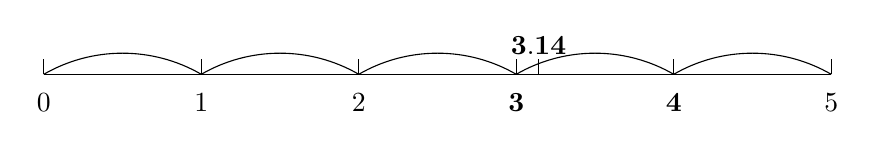
\begin{tikzpicture}[scale=2.0]
        \coordinate (O) at (0,0);
        \coordinate (I) at (1,0);
        \coordinate (II) at (2,0);
        \coordinate (III) at (3,0);
        \coordinate (IV) at (4,0);
        \coordinate (V) at (5,0);

        \coordinate (PI) at (3.1415926,0);

        \node [label={below:$0$}] at (O) {};
        \node [label={below:$1$}] at (I) {};
        \node [label={below:$2$}] at (II) {};
        \node [label={below:$\mathbf{3}$}] at (III) {};
        \node [label={above:$\mathbf{3.14}$}] at (PI) {};
        \node [label={below:$\mathbf{4}$}] at (IV) {};
        \node [label={below:$5$}] at (V) {};

        \draw (O) -- (I) -- (II) -- (III) -- (IV) -- (V);
        \draw (O) -- ++(0,0.1);
        \draw (I) -- ++(0,0.1);
        \draw (II) -- ++(0,0.1);
        \draw (III) -- ++(0,0.1);
        \draw (PI) -- ++(0,0.1);
        \draw (IV) -- ++(0,0.1);
        \draw (V) -- ++(0,0.1);

        \draw (O) arc (120:60:1);
        \draw (I) arc (120:60:1);
        \draw (II) arc (120:60:1);
        \draw (III) arc (120:60:1);
        \draw (IV) arc (120:60:1);
    \end{tikzpicture}
    \caption{Minh họa thuộc tính Archimedes với $x = 3.14$.}
\end{figure}

\begin{theorem}[Phần nguyên của số thực\index{Phần nguyên của số thực}]
    Với mọi số thực $x$, tồn tại duy nhất số nguyên $n$ sao cho $n\leq x < n+1$.

    \noindent Nói riêng, số nguyên $n$ như vậy được gọi là \textbf{phần nguyên của số thực $x$} và được kí hiệu là $\floor{x}$.
\end{theorem}

\begin{proof}
    Theo thuộc tính Archimedes, tồn tại số nguyên $a$ và $b$ sao cho $x < b$ và $-x < a$, kéo theo $-a < x < b$.

    Theo tính chất bắc cầu của quan hệ thứ tự trên tập hợp số thực, nếu một số nguyên $c$ thỏa mãn $c\leq x$ thì $c\leq b$. Theo nguyên lý thứ tự tốt, tập hợp các số nguyên nhỏ hơn hoặc bằng $x$ có phần tử lớn nhất, chúng ta kí hiệu phần tử đó là $n$. Vì $n < n + 1$ và $n + 1$ là một số nguyên nên theo định nghĩa của $n$, chúng ta có $n\leq x < n + 1$.

    Giả sử số nguyên $m$ thỏa mãn $m\leq x < m + 1$. Giả sử phản chứng rằng $m < n$, khi đó $m + 1\leq n$, kéo theo $m + 1\leq x$, mâu thuẫn với $x < m + 1$. Giả sử phản chứng rằng $n < m$, khi đó $n + 1\leq m$, kéo theo $n + 1\leq x$, mâu thuẫn với $x < n + 1$. Do đó $m = n$.

    Vậy với mọi số thực $x$, tồn tại duy nhất số nguyên $n$ sao cho $n\leq x < n+1$.
\end{proof}

\begin{theorem}[Tính trù mật của tập hợp số hữu tỉ\index{Tính trù mật của tập hợp số hữu tỉ}]
    Với mọi số thực $x, y$ sao cho $x < y$, tồn tại số hữu tỉ $q$ sao cho $x < q < y$.
\end{theorem}

\begin{proof}
    Theo thuộc tính Archimedes, tồn tại số nguyên $n$ sao cho $1 < n(y - x)$. Do đó $1 + nx < ny$. Theo định nghĩa phần nguyên của số thực, chúng ta có $nx < \floor{nx} + 1 \leq nx + 1 < ny$.

    Do đó, với số nguyên $m = \floor{nx} + 1$, chúng ta có $nx < m < ny$. Bên cạnh đó, vì $y - x > 0$ và $n > 0$ nên  $1 < n(y - x)$ kéo theo $n > 0$. Do đó $x < \frac{m}{n} < y$.

    Vậy, với mọi số thực $x, y$ sao cho $x < y$, tồn tại số hữu tỉ $q$ sao cho $x < q < y$.
\end{proof}

\subsection{Bài tập}

\section{Số phức}

\subsection{Xây dựng tập hợp số phức}

\subsection{Phần thực, phần ảo, liên hợp của số phức}

\subsection{Biểu diễn hình học và dạng lượng giác của số phức}

\subsection{Bài tập}
